\documentclass[presentation]{beamer}
\usepackage{common}

\title[\lecturecode{07}]{07 \\ Functions in C\# \\ delegates, lambdas, and FP ideas}

\author[Mirko Viroli]{Mirko Viroli}
\institute[]{\texttt{mirko.viroli@unibo.it}}

\begin{document}

\frame[label=coverpage]{\titlepage}
\newcommand{\codepath}[1]{../../code/lecture-07/#1}

\section{FP and OOP}

\fr{Programming paradigms}{
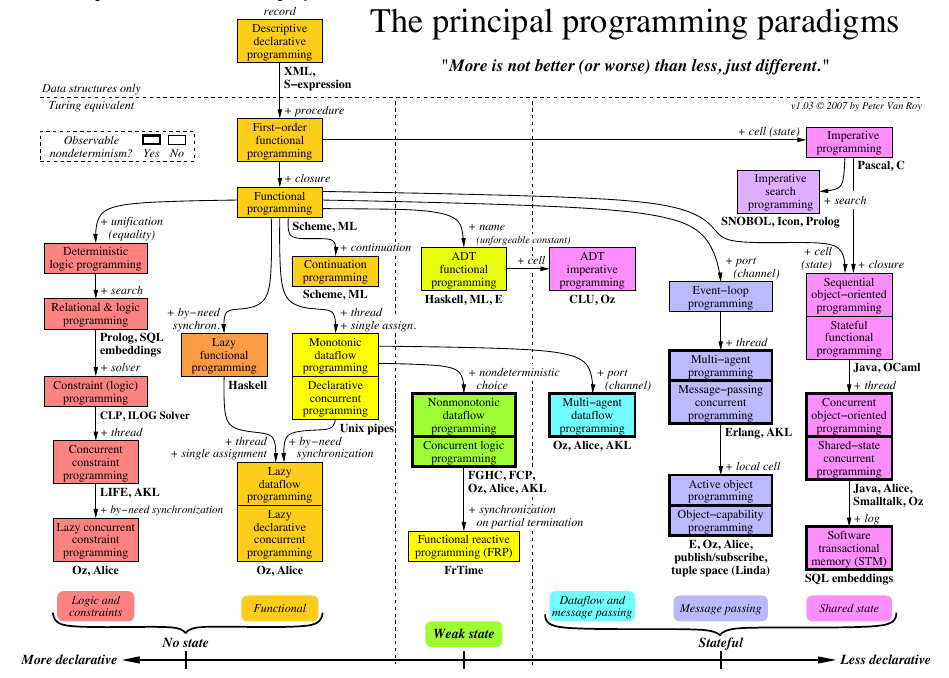
\includegraphics[height=0.9\textheight]{img/para.png}
}



\fr{Main paradigms: Imperative languages}{
   \bl{Motto}{
      {\Large First do this, then do that}
   }
   \bl{Elements}{\iz{
      \item computing as executing statements that change a program state
      \item structured programming constructs (for, while) help control
      \item known to be the most ``natural'' approach for beginners
      \item inspired by hardware aspects
      \item concepts: instructions, procedures, modules
      \item also the starting point for OO
   }}
   \bl{Examples}{\iz{
      \item Fortan, Algol, Pascal, Basic, C
   }}
}

\fr{Main paradigms: Object-oriented languages}{
   \bl{Motto}{
      {\Large Send a message to an object to simulate a real-world event}
   }
   \bl{Elements}{\iz{
      \item computing as letting a bunch of objects exchange messages
      \item objects encapsulate data and behaviour
      \item known to be the most ``powerful'' general-purpose approach
      \item concepts: objects, classes, methods, fields
      \item typically, method bodies following the imperative style
   }}
   \bl{Examples}{\iz{
      \item C++, Java, C\#
   }}
}


\fr{Main paradigms: Functional languages}{
   \bl{Motto}{
      {\Large Evaluate an expression and use the resulting value for other evaluations}
   }
   \bl{Elements}{\iz{
      \item computing as applying functions without side effects
      \item recursion used instead of iteration
      \item known to be the most ``elegant'' approach for experts
      \item inspired by mathematics, and theory of lambda-calculus
      \item lately mixed with OOP
   }}
   \bl{Examples}{\iz{
      \item Haskell, F\#, Erlang, ML, Scheme, Lisp
   }}
   }


\frs{5}{Isn't OOP enough?}{
   \bl{Limits of pure OO approaches}{\iz{
      \item ``everything is an object'' can be verbose, and not ``fitting''
      \item several recurrent problems to be solved by ``1 method''-classes (so-called, functional interfaces), which is verbose
      \item (note that verbosity implies inertia in usage)
      \item not declarative: very difficult to abstract key behavioural elements from unnecessary implementation details
   }}
   \bl{How can ``functional programming'' ideas help OOP?}{\iz{
      \item a smooth abstraction for computing information
      \item nice techniques to abstract imperative aspects
      \item nice techniques to support concurrency orthogonally
      \item higher confidence in the correctness of code
      \item[$\Rightarrow$] possible disadvantage for software engineering: \\
      functional code is terser and requires some advanced competence
   }}
}

\fr{Functional ideas outside functional languages}{
   \bl{Ideas of functional languages, recently brought e.g. in OO languages}{\iz{
    \item prefer immutability
    \item methods should better either change state or compute/return information
    \item methods should better be single expressions/statements
    \item separate construction logic from classes (see factory pattern)
    \item use of functions/lambdas as values (see strategy pattern)
    \item use of lazy-evaluation in data structures (see iterator)
    \item focus on ``what'' and not on ``how''
   }}
}

\section{Functional strategies}

\fr{Scenarios for functional strategies}{
    \bl{Examples}{\iz{
        \item Abstraction: code seems to contain ``out-of-place'' details
        \item Extendibility: code seems to require adjustments from the start
        \item Reusability: code seems an instance of a general problem
    }}
    \bl{Typically ``one-for-all'' solution: functioanl strategy}{\iz{
        \item extract the detail into an interface with single method
        \item such method is used just as a function
        \item many implementations could be smoothly provided 
    }}
}

\fr{\Cil{BankAccount} scenario}{
  \codeview{1}{6}{36}{\tiny}{\codepath{BankAccount/Program.cs}}
}


\fr{\Cil{BankAccount} implementation}{
  \codeview{1}{38}{67}{\tiny}{\codepath{BankAccount/Program.cs}}
}


\frs{5}{First spot: generalising using \Cil{IComparer<T>}}{
  \bl{Generalising \cil{Richest} into a reusable algorithm}{\iz{
    \item \cil{Richest} is just a \cil{Max} with a specific criteria
    \item should abstract over \cil{>}
    \item we pass instead an object with competence of comparing \cil{IBankAccounts}
    \item such a competence is modelled by a \cil{int Compare<T>(T t1, T t2)} method
    \item the client of the API should properly create a suitable comparer.
  }}
  \bl{\cil{IComparer<T>}}{\iz{
    \item widely used in libraries, e.g. \cil{List<T>.Sort}
  }}
  \bl{A note on contravariance}{\iz{
    \item what would be a possible variance for \cil{Compare}?
    \item how would it be useful?
  }}
}

\fr{Using \Cil{Compare<T>}}{
  \codeview{1}{32}{57}{\tiny}{\codepath{BankAccountComparer/Program.cs}}
}

\fr{Calling \Cil{Max<T>}}{
  \codeview{1}{6}{31}{\tiny}{\codepath{BankAccountComparer/Program.cs}}
}

\frs{5}{Other spots in \Cil{BankAccount}}{
  \bl{Abstracting a \cil{IFeeCalculator}}{\iz{
    \item the hypothesis that withdrawal fee is $1$ appears weak
    \item surely this has to be generalise
    \item it could vary across different accounts
    \item it could vary dependning on the actual amount
    \item could introduce an interface \cil{IFeeCalculator}
  }}
  \bl{Abstracting a \cil{IWithdrawalAction}}{\iz{
    \item what should we do if withdrawal fail?
    \item surely that task is better left to a different class
    \item in this case, perhaps many different behaviour have to be defined
    \item shuold abstract from that specific behaviour
    \item could introduce an interface \cil{IWithdrawalAction}
  }}
  
}


\fr{Interfaces}{
  \codeview{1}{14}{44}{\tiny}{\codepath{BankAccountStrategies/Program.cs}}
}

\fr{\Cil{FlexibleBankAccount}}{
  \codeview{1}{46}{75}{\tiny}{\codepath{BankAccountStrategies/Program.cs}}
}

\fr{\Cil{UseFlexibleBankAccount}}{
  \codeview{1}{77}{98}{\tiny}{\codepath{BankAccountStrategies/Program.cs}}
}

\section{C\# delegates and anonymous functions}

\fr{Improving functional strategies}{
    \bl{Functional strategies}{\iz{
        \item a specific case of the so-called Strategy pattern
        \item if introduces substantial ``boilerplate code'': an additional interface, one or more implementing classes, the need of creating an object when the strategy is to be defined
        \item the whole idea is actually simply that of a ``function''
    }}
    \bl{The C\# path across time how to instantiate a delegate}{\iz{
        \item wrapping method references (C\# 1.0)
        \item anonymous functions (C\# 2.0)
        \item lambdas (C\# 3.0) -- the one suggested now
    }}
}

\frs{10}{C\# delegates}{
    \bl{Delegate}{\iz{
        \item a delegate is a wrapper for a method (reference) of a specific type (input/output arguments)
        \item defining a delegate \cil{D} means to define one such type and giving it a name
        \item syntax: \cil{delegate <ret-type> D(<parameters list>);}
        \item ``under the hood'' this is just a subclass of \cil{System.Delegate}
    }}
    \bl{Instantiation of a delegate by method reference}{\iz{
        \item if there is a method \cil{M} (static or instance) accessible in scope
        \item you can define a variable of type \cil{D} assigned to method \cil{M}
        \item syntax: \cil{D del = new D(M);}, or simply passing \cil{M} where a \cil{D} is expected
    }}
    \bl{Call of a delegate}{\iz{
        \item given the above definition, simply \cil{del} is like a method to be called
    }}
    \bl{Multichannel delegates}{\iz{
        \item given two delegates that return void (also called \alert{even delegates}), they can be combined by operators \cil{+}, \cil{-}, \cil{+=}, \cil{-=}
    }}
}


\fr{Definition and use of delegates}{
  \codeview{1}{13}{43}{\tiny}{\codepath{BankAccountDelegates/Program.cs}}
}

\fr{Instantiation of delegates}{
  \codeview{1}{45}{75}{\tiny}{\codepath{BankAccountDelegates/Program.cs}}
}

\fr{Anonymous functions}{
    \bl{Pros and cons of delegates}{\iz{
        \item surely reduce boilerplace code, and are hence more convenient than using interfaces
        \item still there's boilerplate code, since a method is needed somewhere to implement your functional strategy, even if short
        \item recalling that a functional strategy is just a ``function'' (in a mathematical/computational interpretation)...
        
    }}
    \bl{Anonynous functions}{\iz{
        \item a mechanism to express ``in-line'' a function to be passed where a delegate is expected
        \item syntax of expression: \cil{delegate(<parameters list>)\{<body>\}}, to be passed where a compatible delegate is expected
        \item essentially, it is a function without name and with keyword \cil{delegate} upfront
    }}
}

\fr{Using anonymous function}{
  \codeview{1}{16}{47}{\tiny}{\codepath{BankAccountAnonymous/Program.cs}}
}

\frs{5}{Lambda expressions}{
    \bl{Pros and cons of anonymous functions}{\iz{
        \item surely further reduce boilerplace code, and are hence more convenient than using method references
        \item still there's boilerplate code, since the syntax is still rather long: one would more heavility rely on inference and on single-expression body
        \item lambda-expressions have been invented in 1930 by Alonso Church
        \item Scala language started using them in OOP languages, and now also Java have them
    }}
    \bl{Lambda-expression}{\iz{
        \item Complete syntax: \cil{(T1 x1,...,Tn xn) => \{<body>\}}
        \item With inference: \cil{(x1,...,xn) => \{<body>\}}
        \item With single-expression body: \cil{(T1 x1,...,Tn xn) => <exp>}
        \item With single argument and inference: \cil{x => \{<body>\}}
        \item With unused inputs: \cil{(_,...,_) => \{<body>\}}
        \item ...and combinations
        \item[$\Rightarrow$] should generally use the shortest version possible
    }}
}

\fr{Using lambdas}{
  \codeview{1}{9}{37}{\tiny}{\codepath{BankAccountLambdas/Program.cs}}
}

\frs{10}{Reusable delegates in libraries}{
    \bl{Generic functions in namespace \cil{System}}{\iz{
        \item \cil{delegate TResult Func<out TResult>(); }
        \item \cil{delegate TResult Func<in T, out TResult(T arg); }
        \item \cil{delegate TResult Func<in T1, in T2, out TResult(T1 arg1, T2 arg2); }
        \item \dots
        \item \cil{delegate bool Predicare<in T>(T obj)}
    }}
    \bl{Generic actions in namespace \cil{System}}{\iz{
        \item \cil{delegate void Action(); }
        \item \cil{delegate void Action<in T>(T obj); }
        \item \cil{delegate void Action<in T1, in T2>(T1 obj1, T2 obj2); }
        \item \dots
    }}
    \bl{Guideline}{\iz{
        \item define your own delegates only if domain-specific
        \item otherwise, consider using  library delegates
    }}
}

\fr{\Cil{BankAccount} with \Cil{Func} and \Cil{Action}}{
  \codeview{1}{14}{40}{\tiny}{\codepath{BankAccountFunc/Program.cs}}
}

\fr{Use \Cil{BankAccount} with \Cil{Func} and \Cil{Action}}{
  \codeview{1}{42}{66}{\tiny}{\codepath{BankAccountFunc/Program.cs}}
}

\fr{Exercise with \Cil{Func}, \Cil{Predicate} and \Cil{Action}}{
  \codeview{1}{7}{35}{\tiny}{\codepath{ExercisesWithFunc/Program.cs}}
}

\fr{Solution for the first three}{
  \codeview{1}{37}{59}{\tiny}{\codepath{ExercisesWithFunc/Program.cs}}
}

\fr{Expectations}{
  \codeview{1}{61}{81}{\tiny}{\codepath{ExercisesWithFunc/Program.cs}}
}


\fr{A preview of standard LINQ library}{
    \codeview{1}{28}{56}{\tiny}{\codepath{LINQExample/Program.cs}}
}

\fr{The used \Cil{Person} class}{
  \codeview{1}{7}{26}{\tiny}{\codepath{LINQExample/Program.cs}}
}



\section{Other recipes of functional programming}

\fr{Prefer immutability}{
    \codeview{1}{8}{40}{\tiny}{\codepath{PreferImmutability/Program.cs}}
}

\fr{Make defensive copies}{
    \codeview{1}{7}{38}{\tiny}{\codepath{DefensiveCopy/Program.cs}}
}


\fr{Consider static factories instead of constructors}{
  \codeview{1}{5}{36}{\tiny}{\codepath{PreferStaticFactories/Program.cs}}
}


\frs{5}{Hide implementations: only make available types}{
    \bl{The \cil{IOption<T>} case: a common functional block}{\iz{
        \item it represents information possibly not available
        \item note construction and hiding
    }}
    \codeview{1}{7}{30}{\tiny}{\codepath{NoExceptions/Program.cs}}
}

\fr{Don't abuse exceptions: use designed abstractions instead}{
    \codeview{1}{32}{52}{\tiny}{\codepath{NoExceptions/Program.cs}}
}


\end{document}

\fr{Many languages, few paradigms}{
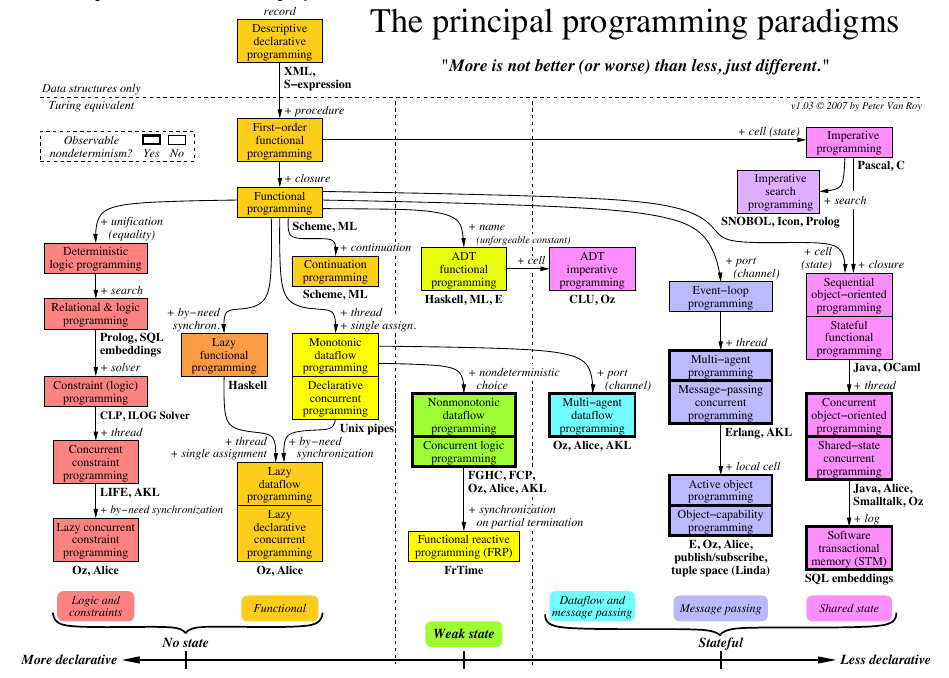
\includegraphics[height=0.9\textheight]{img/para.png}
}


\fr{Uniform abstractions with classes}{
  \bl{Uniform abstractions for recurring problems}{\iz{
    \item During the development of various systems, recurrent problems are encountered that can find a common solution
    \item In some cases these solutions are factorisable (by abstraction) into a single highly reusable class
  }}
  \bl{A fundamental case: the \alert{collection}}{\iz{
    \item A collection is an object whose task is to store the reference to a (typically unspecified) number of other objects
    \item Among its tasks is to allow modifications and quick access to the set of elements of this collection
    \item Various strategies can be used, following the theory/practice of algorithms and data structures
  }}
}

\frs{5}{An example: \Cil{IntVector}}{
  \bl{Collection \Cil{IntVector}}{\iz{
    \item Contains numerical series (vectors) of unknown, variable/dynamic size
    \item Implementation idea: composing an array, expanded/changed as needed
  }}
  \fg{height = 0.6 \textheight}{img/uml-int-vector-pre.pdf}
}

\fr{Preliminary \Cil{UseIntVector}}{
  \codeview{1}{5}{21}{\scriptsize}{\codepath{IntVectorPre/Program.cs}}
}

\fr{Preliminary \Cil{IntVector}}{
  \codeview{1}{23}{53}{\tiny}{\codepath{IntVectorPre/Program.cs}}
}

\frs{5}{C\# Indexers}{
    \bl{Let's improve this design a bit}{\iz{
        \item we have getters/setters that are parametric, namely, they depend on an indexer
        \item we would like to handle them as we would with properties
    }}
   \bl{C\# Indexer}{\iz{
        \item a sort of parametric property
        \item it has no name 
        \item it supports the array access notation for reading and/or writing elements
        \item basic syntax: \cil{public <type> this[<type> <name>]\{ get\{...\} set\{...\}\}}
        \item could have many parameters of the indexer
        \item could have many indexers in a class, with different parameters
    }}
}

\frs{5}{\Cil{IntVector} (with indexer)}{
  \codeview{1}{19}{51}{\tiny}{\codepath{IntVector/Program.cs}}
}

\fr{\Cil{UseIntVector}}{
  \codeview{1}{5}{17}{\scriptsize}{\codepath{IntVector/Program.cs}}
  \bx{In this lesson we shall assume we never ``escape'' boundaries of arrays and collections, which would result in exceptions} 
}

\frs{5}{UML: \Cil{IntVector}}{
  \fg{height = 0.6 \textheight}{img/uml-int-vector.pdf}
}


\frs{5}{A first step towards uniformity}{
  \bl{Only vectors of \cil{int}?}{\iz{
    \item Experience would immediately lead to the need to design vectors of \cil{double}, \cil{bool}, \dots that is, of any value type
    \item And then, also vectors of \cil{String}, \cil{DateTime}, and so on
    \item The implementation would be similar, but without the possibility of reuse.
  }}
  \bl{The idea of ``monomorphic'' collections}{\iz{
    \item A first solution to the problem is obtained by exploiting inclusive polymorphism and the ``everything is an object'' philosophy (including the use of autoboxing)
    \item Only a \cil{ObjectVector} is created, simply by replacing \cil{int} with \cil{object}
    \item Any element is inserted (via implicit upcast conversions)
    \item When you get a value back you need an explicit downcast with \cil{as} operator
    \item Working with such interfaces gets bloated, and low-level
  }}
}

\fr{From \Cil{IntVector} to \Cil{ObjectVector}}{
  \fg{height = 0.6 \textheight}{img/uml-obj-vector.pdf}
}

\fr{\Cil{UseObjectVector}}{
  \codeview{1}{5}{32}{\ssmall}{\codepath{ObjectVector/Program.cs}}
}

\frs{5}{\Cil{ObjectVector}}{
  \codeview{1}{34}{66}{\tiny}{\codepath{ObjectVector/Program.cs}}
}

\fr{Another example of collection: \Cil{ObjectList}}{
  \codeview{1}{25}{47}{\ssmall}{\codepath{ObjectList/Program.cs}}
}

\fr{\Cil{UseObjectList}}{
  \codeview{1}{6}{23}{\ssmall}{\codepath{ObjectList/Program.cs}}
}

\fr{The need for a parametric polymorphism approach}{
  \bl{In C\# 1.0}{\iz{
    \item This was the standard approach to building collections
  }}
  \bl{Problem}{\iz{
    \item With this approach, C\# code resulted in many uses of objects similar to \cil{ObjectVector} or \cil{ObjectList}
    \item It was very easy to lose track of what the content was \dots {\iz{
      \item which objects a collection contain? only \cil{int}? only \cil{strings}?
    }}
    \item The code often contained bad conversions
  }}
  \bl{More generally}{
    The problem arises every time I want to collect objects whose type is not known a priori, but could be subject to inclusive polymorphism
  }
}

% \fr{The problem with multiple compositions}{
% \sizedcode{\ssmall}{09 / code / LampsRow.java}
%}

\section{Generic classes and methods}

\fr{Parametric polymorphism}{
  \bl{Basic idea: generification}{\iz{
    \item Given a code snippet \cil{F} that works on a certain type, say \cil{string}, if it could also work uniformly with others\dots
    \item \dots you make it parametric by replacing \cil{string} with a sort of \cil{T} variable (called \alert{type-variable}, i.e. a variable that contains a type)
    \item At this point, when you need the code fragment instantiated on the strings, you use \cil{F<String>}, that is, it is required that \cil{T} becomes \cil{string}
    \item When you need the code snippet instantiated on integers, use \cil{F<int>}
  }}
  \bl{C\# Generics}{\iz{
    \item Generic classes / interfaces / methods
    \item Fully integrated in the type system and run-time (differently from other frameworks, like the JVM)
  }}
}

\fr{A generic class for lists}{
  \codeview{1}{24}{46}{\ssmall}{\codepath{GenericList/Program.cs}}
}

\fr{Using a generic class}{
  \codeview{1}{5}{22}{\ssmall}{\codepath{GenericList/Program.cs}}
}

\frs{5}{Terminology, and essential elements}{
  \bl{Given a generic class \cil{C <T1, T2>} ..}{\iz{
    \item \cil{T1} and \cil{T2} are called its \alert{type-variables}
    \item \cil{T1} and \cil{T2} can be used as any type within the class
  }}
  \bl{Clients of generic classes}{\iz{
    \item Must use \alert{generic types}: ``instantiated'' versions of generic classes \iz{
      \item \cil{C<String, Integer>}, \cil{C<C<Object, Object>, Object>}
      \item Can't use \cil{C} without type parameters
    }
    \item Each type-variable must be replaced with an actual type, i.e. with a \alert{parameter}, which can be{\iz{
      \item a (non-generic) class, e.g. \cil{Object}, \cil{String}, ..
      \item a defined type-variable, e.g. \cil{T1, T2} (used inside the \cil{C <T1, T2>} class)
      \item a fully instantiated generic type, e.g. \cil{C <Object, Object>}
      \item .. or partially instantiated, e.g. \cil{C <Object, T1>} (in \cil{C<T1, T2>})
      \item a value type: \cil{int}, \cil{double}, \cil{bool}
    }}
  }}
}

\frs{5}{Generic vector}{
  \codeview{1}{33}{65}{\tiny}{\codepath{GenericVector/Program.cs}}
}

\fr{Using generic vector}{
  \codeview{1}{5}{31}{\ssmall}{\codepath{GenericVector/Program.cs}}
}

\section{Generic Methods}

\fr{Generic Methods}{
  \bl{Basic idea}{\iz{
    \item generify a single method in the type(s) of some of its arguments/return
    \item syntactically: add type parameter after method name
    \item at the call side: specify type parameter after method name
    \item at the call side: use type inference, simply avoiding any specification
  }}
  \bl{Two typical applications}{\iz{
    \item generic static methods: as helpers working on generic structures
    \item in generic classes: as a helper to mix differen instantiations
  }}
}

\fr{Generic static methods}{
    \codeview{1}{7}{34}{\ssmall}{\codepath{GenericMethods/Program.cs}}
}

\fr{Generic instance methods: the case of class \Cil{Pair<TA,TB>}}{
  \codeview{1}{35}{51}{\ssmall}{\codepath{Pair/Program.cs}}
}

\fr{Using pairs}{
  \codeview{1}{6}{33}{\ssmall}{\codepath{Pair/Program.cs}}
}


\fr{The advantages of generics}{
  \bx{With generics, C\# becomes a much more expressive language!}
  \bl{Disadvantages}{\iz{
    \item The language is a bit more sophisticated, and therefore complex
    \item If not used well, they can undermine the comprehensibility of the software
    \item They should not be abused!!
  }}
  \bl{Advantages - if used well}{\iz{
    \item More understandable code
    \item More possibilities for reuse of functionality (almost obligatory now)
    \item Safer code - the compiler reports errors that are difficult to find otherwise
  }}
}

\section{Generic interfaces}

\frs{10}{Generic interfaces}{
  \bl{What is a generic interface}{\iz{
    \item It is an interface that declares type-variables: \cil{interface I <T1, T2> \{.. \}}
    \item The type-variables appear in the methods signatures defined by the interface
    \item When a class implements it, it must instantiate the type variables (or assign them to other type-variables if it is generic)
  }}
  \bl{Uses}{
    To create uniform contracts that do not have to depend on the types used
  }
  \bl{Example 1}{\iz{
    \item An \cil{IGenericVector<T>} would be use to abstract over \cil{GenericVector<T>}
  }}
  \bl{Example 2: a new case, \alert{Iterators}}{\iz{
    \item An iterator is an object used to access a sequence of elements
    \item We will now look at a simplified version - different from that of the Java libraries
  }}
}

\fr{\Cil{IGenericVector<T>}}{
  \codeview{1}{20}{27}{\footnotesize}{\codepath{IGenericVector/Program.cs}}
}

\frs{5}{Implementing \Cil{IGenericVector}}{
  \codeview{1}{29}{61}{\tiny}{\codepath{IGenericVector/Program.cs}}
}

\section{Iterators and collections}

\frs{10}{The Iterator pattern}{
    \bl{Idea}{\iz{
        \item Assume an object represents a set of values {\iz{
            \item a collection, a source of information, a mathematical set,\dots
        }}
        \item \dots how could it give a service to let clients retrieve all such values?
        \item Iterator pattern: the object gives to requestors a so-called \alert{iterator}
        \item An iterator is an object with a method to extract the ``next'' element of the set, to be called iteratively until there are othe objects available
        \item various implementations possible
    }}
    \bl{Iterator core support in C\#}{\iz{
        \item interface \cil{IEnumerable<T>}: the root of the collection library{\iz{
            \item can use it  in \cil{foreach} construct
        }}
        \item interface \cil{IEnumerator<T>}: the actual iterator you can ask to a \cil{IEnumerable}
        \item both interfaces are connected with the \cil{yield return} construct
    }}
    
}

\fr{\Cil{IEnumerator<T>}, and \Cil{Range} example}{
  \codeview{1}{9}{19}{\ssmall}{\codepath{Enumerables/Enumerators.cs}}
  \codeview{1}{22}{33}{\ssmall}{\codepath{Enumerables/Enumerators.cs}}
}

\fr{\Cil{RangeEnumerator} implementation}{
  \codeview{1}{35}{64}{\tiny}{\codepath{Enumerables/Enumerators.cs}}
}

\fr{The actual enumerable: \Cil{Range}}{
  \codeview{1}{32}{43}{\ssmall}{\codepath{Enumerables/Enumerables.cs}}
}

\fr{Using \Cil{Range} with \Cil{IEnumerator}}{
  \codeview{1}{7}{30}{\ssmall}{\codepath{Enumerables/Enumerables.cs}}
}

\fr{\Cil{foreach} is compatile with \Cil{IEnumerable}s!}{
  \codeview{2}{20}{35}{\ssmall}{\codepath{Enumerables/Program.cs}}
}

\frs{5}{The \Cil{yield return} construct}{
  \codeview{1}{34}{62}{\ssmall}{\codepath{YieldReturn/Program.cs}}
}

\fr{The \Cil{yield return} construct}{
  \codeview{1}{6}{32}{\ssmall}{\codepath{YieldReturn/Program.cs}}
}


\fr{Creating a vector as an \Cil{IEnumerable<T>}}{
  \codeview{1}{23}{51}{\ssmall}{\codepath{EnumerableVector/Program.cs}}
}

\fr{Enumerating our vector}{
  \codeview{1}{7}{21}{\ssmall}{\codepath{EnumerableVector/Program.cs}}
}

\fr{\Cil{IEnumerable<T>} and collections}{
  \bl{The collection framework very briefly (will be explored next)}{\iz{
    \item various implementations available for collecting data
    \item all implement interface \cil{IEnumerable<T>}
    \item all have standard methods \cil{Add}, indexers, and  so on
  }}
  \codeview{1}{6}{22}{\ssmall}{\codepath{Collections/Program.cs}}
}

\fr{An example application: \Cil{ClassManagement}}{
  \codeview{1}{7}{35}{\tiny}{\codepath{ClassManagement/Program.cs}}
}

\frs{5}{An example application: \Cil{ClassManagement}}{
  \codeview{1}{37}{69}{\tiny}{\codepath{ClassManagement/Program.cs}}
}

\section{Constrained Polymorphism}

\frs{10}{Constrained Polymorphism}{
    \bl{Consider a generic class \cil{C<T>} or method \cil{M<T>(...)}}{\iz{
        \item what operations are we allowed to perform on elements of type \cil{T}?
        \item we can only assume it is an \cil{object}, hence e.g. \cil{ToString}
        \item how can we express something more?
    }}
    \bl{\cil{where} clauses in type parameters}{\iz{
        \item \cil{where T : class}: used to mean that \cil{T} should be a reference type
        \item \cil{where T : new()}: used to mean that \cil{T} must have a 0-ary constructor
        \item \cil{where T : Lamp}: used to mean that \cil{T} must be a subtype of \cil{Lamp} class
        \item \cil{where T : ILamp}: used to mean that \cil{T} must be a subtype of \cil{ILamp} interface
        \item \cil{where T : U}: used to mean that \cil{T} must be a subtype of another type parameter \cil{U}
    }}
}

\frs{5}{Examples of Constrained Polymorphism}{
  \codeview{1}{7}{39}{\tiny}{\codepath{Constrained/Program.cs}}
}

\section{Variance}

\fr{Deepening: on the substitutability of generics}{
  \bl{Question: \cil{List<string>} is a subtype of \cil{List<object>}?}{
    That is, can we think of passing a \cil{List<string>} in all contexts where a \cil{List<object>} is expected instead?
  }
    \bl{Answer: no!! It would seem so .. but:}{
    what happens if in the method below we pass a \cil{List<string>}? \\
    $\Rightarrow$ we could easily compromise the integrity of the list
  }
  \codeview{1}{8}{18}{\tiny}{\codepath{VarianceProblem/Program.cs}}
}

\frs{5}{Subtyping and safety}{
  \bl{\alert{Safety} of an OO language}{
    If no combination of instructions leads to being able to invoke a method on an object whose class does not define it{\iz{
      \item Subtyping must follow the principle of substitutability
    }}
    More generally, we seeks for limiting language errors at runtime.
  }
  \bl{C\#}{\iz{
    \item It has the goal of being safe whenever possible
    \item Therefore, it correctly prevents \cil{List<string> <: Vector<object>}, even though \cil{string <: object}
  }}
  \bl{Generic and safety}{
    In general, different instances of a generic class are disconnected
    \iz{
    \item there is no \alert{covariance}: it is not true that \cil{C<T> <: C<S>} with \cil{T <: S}
    \item there is no \alert{contravariance}: it is not true that \cil{C<S> <: C<T>} with \cil{T <: S}
  }}
}

\fr{Unsafety with C\# arrays}{
  \bl{C\# arrays are treated as covariants!}{\iz{
    \item Arrays look a lot like a generic type
    \item \cil{string[]} $ \sim $ \cil{List<string>}, \cil{T[]} $ \sim $ \cil{List<T>}
    \item And so we know it wouldn't be safe to handle them with covariance
    \item But in C\# it is exactly like this!! E.g. \cil{string[] <: object[]}
    \item So any write to array could potentially fail .... throwing an exception
  }}
  \codeview{1}{7}{17}{\tiny}{\codepath{VarianceArrays/Program.cs}}
}

\frs{10}{Covariance and access operations}{
  \bl{Covariance (\cil{C<T> <: C<S>} with \cil{T<:S}) would be admissible if:}{\iz{
    \item The \cil{C<X>} class had no operations receiving \cil{X} objects
    \item That is, it has only private or readonly fields and no methods with \cil{X} as argument
  }}
  \bl{Contravariance (\cil{C<S> <: C<T>} with \cil{T <: S}) would be admissible if:}{\iz{
    \item The \cil{C<X>} class had no operations that produce \cil{X} objects
    \item That is, it has only private fields and no method with return type \cil{X}
  }}
  \bl{In practice:}{\iz{
    \item Most of the generic \cil{C<X>} classes have fields of type \cil{X} (composition) and getter and setter operations, and therefore their covariance and contravariance would not work
    \item C\# allows indication of covariance or contravariance in generic interfaces for which it is safe to do so, by keywords \cil{in} and \cil{out}
    \item this allows to nicely deal with reusability of generic methods, as will see in the collection framework
  }}
}

\fr{An advanced example of ``variant'' modelling}{
\codeview{1}{8}{26}{\ssmall}{\codepath{VariantVector/Program.cs}}
}

\fr{Expectation}{
\codeview{1}{58}{72}{\tiny}{\codepath{VariantVector/Program.cs}}
}

\fr{Straightforward implementation}{
\codeview{1}{27}{56}{\tiny}{\codepath{VariantVector/Program.cs}}
}
\end{document}






\end{document}


